%% bare_jrnl.tex

\documentclass[journal]{IEEEtran}

\usepackage{cite}
\usepackage{graphicx}
\graphicspath{{images/}}
\DeclareGraphicsExtensions{.png,.jpg,.pdf}
\usepackage{ifpdf}
\usepackage{cite}
\usepackage{todonotes}
\usepackage{siunitx}

\ifCLASSINFOpdf
  % \usepackage[pdftex]{graphicx}
  % declare the path(s) where your graphic files are
  % \graphicspath{{../pdf/}{../jpeg/}}
  % and their extensions so you won't have to specify these with
  % every instance of \includegraphics
  % \DeclareGraphicsExtensions{.pdf,.jpeg,.png}
\else
  % or other class option (dvipsone, dvipdf, if not using dvips). graphicx
  % will default to the driver specified in the system graphics.cfg if no
  % driver is specified.
  % \usepackage[dvips]{graphicx}
  % declare the path(s) where your graphic files are
  % \graphicspath{{../eps/}}
  % and their extensions so you won't have to specify these with
  % every instance of \includegraphics
  % \DeclareGraphicsExtensions{.eps}
\fi

\usepackage[cmex10]{amsmath}
\interdisplaylinepenalty=2500

\usepackage{algorithmic}
\usepackage{array}
\usepackage{mdwmath}
\usepackage{mdwtab}
\usepackage{eqparbox}
\usepackage[tight,footnotesize]{subfigure}
%\usepackage[font=footnotesize]{subfig}
\usepackage{fixltx2e}
\usepackage{color}
\usepackage{mathtools}
\usepackage{color}

% correct bad hyphenation here
\hyphenation{op-tical net-works semi-conduc-tor}

\begin{document}

\title{A New Experimental Setup for Electric Motor Drives Laboratory with Mechanical Load Simulator}

\author{Mesut~U\u{g}ur,~\IEEEmembership{Student~Member,~IEEE,}
        Siamak~P,~\IEEEmembership{Student~Member,~IEEE,}
        and~Ozan~Keysan,~\IEEEmembership{Member,~IEEE}% <-this % stops a space
\thanks{M. U\u{g}ur, Siamak P and O. Keysan are with the Department of Electrical and Electronics Engineering, Middle East Technical University, ankara,
Turkey, 06800, e-mail: ugurm@metu.edu.tr}% <-this % stops a space
\thanks{J. Doe and J. Doe are with Anonymous University.}% <-this % stops a space
\thanks{Manuscript received April 19, 2005; revised August 26, 2015.}}

\markboth{IEEE Transactions on Education,~Vol.~xx, No.~xx, xx~xx}%
{Shell \MakeLowercase{\textit{et al.}}: Bare Demo of IEEEtran.cls for IEEE Journals}

\maketitle

% As a general rule, do not put math, special symbols or citations
% in the abstract or keywords.
\begin{abstract}
In this paper, a new experimental setup for electric motor drive systems laboratory is presented which acts as a simulator for several real-world mechanical loads. The experimental setup contains two three-phase AC electrical machines which are coupled via their shafts, off-the-shelf motor drive units, transducers and data acquisition system, and a control system constructed on Labview. One machine \cite{Wang2017} which is a permanent magnet synchronous machine (PMSM) is used as a generator under torque control to simulate various mechanical load characteristics changing with speed while the other one which is a three-phase induction machine is operated as the motor to be driven by speed control. The main purpose of the experiment is to enable students who are 4th year undergraduates to implement speed control techniques for induction motors and analyze the behavior and characteristics of the motor and the drive while the motor is subjected to different simulated real-world mechanical loads which are difficult and expensive to build in a laboratory such as fan load, pump load, electric traction system etc. During the experiment, the students can observe variation of mechanical output torque, applied voltage and frequency, active and reactive power, efficiency as well as the effects of the motor drive to grid power quality and motor lifetime under these load conditions and make interpretations accordingly.

\end{abstract}

\begin{IEEEkeywords}
electric motor drives, electrical engineering education, laboratory experiments, mechanical load simulator.
\end{IEEEkeywords}


\IEEEpeerreviewmaketitle


\section{Introduction}


\IEEEPARstart{T}{he} key part of an electric motor drive course laboratory is real-world mechanical loads.

65  of the electricity in European Union and 46 of the electricity in the who world is consumed by electric motors. Although not all of these drives contain a dedicated motor drive, considerable amount of applications require adjustable speed drives (ASD). In most of the universities, there exists an undergraduate course related to electric motor drives in electrical engineering departments. It plays a critical role in students' improvement toward being a power engineer or a researcher where the students are taught the significance of energy efficiency, reliability, etc \todo[inline]{burayı bağlayamadım.}

\todo[inline]{Aşağıdaki kısaltmaları bu section'da yapalım}
\textbf{Department of Electrical and Electronics Engineering (DEEE), Middle East Technical University (METU)}

It is desired to have different kinds of mechanical loads in the laboratory to be able demonstrate motor drives' capabilities and limitations. In motor drive applications, most common load types are; pumps, compressors, fans, position controlled automation systems, electric vehicles, railway traction systems, wind-energy systems etc. The significance of motor drive studies is growing every day in today's world. As an example, the share of electric vehicles, which is a typical variable speed motor drive application,   among all vehicles is estimated to be x percent in 20xx.


\todo[inline]{Burada electric vehicle reklamı yapıp örnekler mi versek? Tesla vs.}

\todo[inline]{Multidisciplinary nature of electric motor drives ekleyelim}

\todo[inline]{ASD neden önemli? Kullanılan teknikler neler bahsedelim}



\section{Background of the Electric Motor Drives Course}
The Electric Motor Drives course is a must course for the 4th year undergraduate students which are to complete the requirements of Electrical Machines and Power Electronics area in the DEEE, at METU. The basic content of the course includes basic operating characteristics and classification of electrical drives, solid-state DC and AC motor drive and control techniques, dynamic behavior of electrical machines and selection of drives for various industrial applications. The main objectives of the course are:

\begin{itemize}
\item Understand the fundamental principles of motor drives and the mechanical systems.
\item Analyze and design DC/AC motor drives (including power stage and control loops).
\item Select motor drive systems for various industrial applications.
\item Use multi-domain simulation software.
\item Prepare design reports and use version control system to build online portfolio.
\item Use commercial industrial motor drive systems through laboratory.
\end{itemize}

During the semester, the students are assigned 3 simulation projects which are to be conducted on MATLAB/Simulink to visualize the techniques that they have seen in lectures. Moreover, a hardware motor drive project is assigned at the end of the semester which uses hardware-in-the-loop (HIL) techniques. There have been three experiments with different types of mechanical loads most of which include variable speed driven (VSD) induction motors such as; fan load, pump load and crane-hoist load, as shown in Fig \ref{fig1}. A general block diagram of these setups is also shown in Fig 2.


\todo[inline]{Burada Deneyleri anlatıcaz}

The experiments are as follows:
\begin{itemize}
\item Fan Load Driven by Variable Frequency Drive (VFD)
\item Variable Frequency Drive (VFD) Driven Crane Hoist with Speed Feedback
\item Centrifugal Pump Load Driven by Variable Frequency Drive (VFD)
\item (Demo) Hardware in the loop Motor Drive Controller
\end{itemize}

\begin{figure}[h]
  \centering
  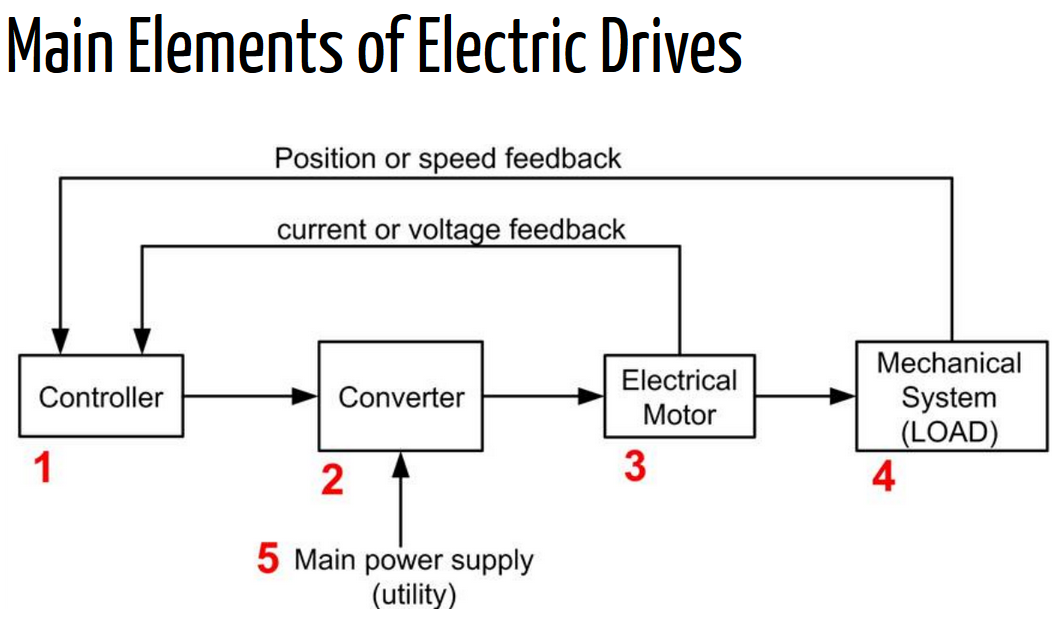
\includegraphics[width=9cm]{blockdia1}
  \caption{Integrated modular motor drive examples}
  \label{fig1}
\end{figure}

Fig.1.

Fig. 2.

Elimizdeki VSD'lerin devre şeması ve blok diyagramı

Deneylerde neler var önemli olarak? Örn: fan yavaşlayınca zor soğuyor.

All of these experimental setups were constructed throughout the years with fundings from several research projects as they require expensive hardware and their installation takes time. With the new experimental setup presented in this paper, it is aimed to create a universal mechanical load simulator in which the torque vs. speed characteristics of the load can be adjusted.



\section{The Experimental Setup}


The experimental setup installed in Middle East Technical University Electrical Machinery Laboratory is shown in figure 1.
As the block diagram of the setup at figure 2 illustrates, the test bench is consist of two electrical machines coupled to each other; an squirrel cage induction machine and a permanent magnet synchronous machine. The IM is supplied through an AC variable frequency drive connected to the grid. The PMSM is drove by a back-to-back AC-DC-AC converter which is also connected to the grid. The back-to-back power converter provides the ability of the two direction power flow to develop a variety of experiments on the setup.
In order to control and monitor the experiment flow LABVIEW interface environment is used on the computer; a supervisory control and data acquisition program provided by National Instruments. An Ethernet connection is used to build a data communication between computer and the drives. The AC drives can be drove with torque or speed reference commands sent by operator of the experiment using the interface program. On the other side, during the experiment a set of data is measured and transmitted to the interface program. A torque transducer placed at the coupling point of IM and PMSM measures and sends the applied torque on the shaft and the rotating shaft speed to the computer. LEM voltage and current transducers are used to gather the electrical variables' data to be monitored at the supplying terminals of the machines. The all data monitoring and test bench controlling job is done via a user interface program seen in figure 3.
Besides a power quality analyzer is connected to the grid connection point of the drives to study the harmonic distortion and the power quality issues.

The experimental setup installed in Middle East Technical University Electrical Machinery Laboratory is shown in figure 1.


\section{Methodology and Aims for Students}

\begin{equation}
\label{eq4}
T_{core} = T_{amb}+p_{c}(T_{core})R_{th,c}
\end{equation}


\section{Results and Interpretation}

Lifetime: high dv/dt
insulation lifetime
additional core losses
Limit on the motor cable length
Filter required. Common mode choke. Use ceramic bearing
Bearing-shaft currents.

Mechanical resonance frequency (bunu labda gördük)


\section{Conclusions}
The conclusion goes here.


\appendices
\section{Proof of the First Zonklar Equation}
Appendix one text goes here.

% you can choose not to have a title for an appendix
% if you want by leaving the argument blank
\section{}
Appendix two text goes here.


% use section* for acknowledgment
\section*{Acknowledgment}


The authors would like to thank...


% Can use something like this to put references on a page
% by themselves when using endfloat and the captionsoff option.
\ifCLASSOPTIONcaptionsoff
  \newpage
\fi



% trigger a \newpage just before the given reference
% number - used to balance the columns on the last page
% adjust value as needed - may need to be readjusted if
% the document is modified later
%\IEEEtriggeratref{8}
% The "triggered" command can be changed if desired:
%\IEEEtriggercmd{\enlargethispage{-5in}}

% references section

% can use a bibliography generated by BibTeX as a .bbl file
% BibTeX documentation can be easily obtained at:
% http://mirror.ctan.org/biblio/bibtex/contrib/doc/
% The IEEEtran BibTeX style support page is at:
% http://www.michaelshell.org/tex/ieeetran/bibtex/
%\bibliographystyle{IEEEtran}
% argument is your BibTeX string definitions and bibliography database(s)
%\bibliography{IEEEabrv,../bib/paper}
%
% <OR> manually copy in the resultant .bbl file
% set second argument of \begin to the number of references
% (used to reserve space for the reference number labels box)
\begin{thebibliography}{1}

\bibitem{IEEEhowto:kopka}
H.~Kopka and P.~W. Daly, \emph{A Guide to \LaTeX}, 3rd~ed.\hskip 1em plus
  0.5em minus 0.4em\relax Harlow, England: Addison-Wesley, 1999.

\end{thebibliography}

% biography section
% 
% If you have an EPS/PDF photo (graphicx package needed) extra braces are
% needed around the contents of the optional argument to biography to prevent
% the LaTeX parser from getting confused when it sees the complicated
% \includegraphics command within an optional argument. (You could create
% your own custom macro containing the \includegraphics command to make things
% simpler here.)
%\begin{IEEEbiography}[{\includegraphics[width=1in,height=1.25in,clip,keepaspectratio]{mshell}}]{Michael Shell}
% or if you just want to reserve a space for a photo:

\begin{IEEEbiography}{Michael Shell}
Biography text here.
\end{IEEEbiography}

% if you will not have a photo at all:
\begin{IEEEbiographynophoto}{John Doe}
Biography text here.
\end{IEEEbiographynophoto}

% insert where needed to balance the two columns on the last page with
% biographies
%\newpage

\begin{IEEEbiographynophoto}{Jane Doe}
Biography text here.
\end{IEEEbiographynophoto}

% You can push biographies down or up by placing
% a \vfill before or after them. The appropriate
% use of \vfill depends on what kind of text is
% on the last page and whether or not the columns
% are being equalized.

%\vfill

% Can be used to pull up biographies so that the bottom of the last one
% is flush with the other column.
%\enlargethispage{-5in}



% that's all folks
\end{document}


% if have a single appendix:
%\appendix[Proof of the Zonklar Equations]
% or
%\appendix  % for no appendix heading
% do not use \section anymore after \appendix, only \section*
% is possibly needed

% use appendices with more than one appendix
% then use \section to start each appendix
% you must declare a \section before using any
% \subsection or using \label (\appendices by itself
% starts a section numbered zero.)
%



% An example of a floating figure using the graphicx package.
% Note that \label must occur AFTER (or within) \caption.
% For figures, \caption should occur after the \includegraphics.
% Note that IEEEtran v1.7 and later has special internal code that
% is designed to preserve the operation of \label within \caption
% even when the captionsoff option is in effect. However, because
% of issues like this, it may be the safest practice to put all your
% \label just after \caption rather than within \caption{}.
%
% Reminder: the "draftcls" or "draftclsnofoot", not "draft", class
% option should be used if it is desired that the figures are to be
% displayed while in draft mode.
%
%\begin{figure}[!t]
%\centering
%\includegraphics[width=2.5in]{myfigure}
% where an .eps filename suffix will be assumed under latex, 
% and a .pdf suffix will be assumed for pdflatex; or what has been declared
% via \DeclareGraphicsExtensions.
%\caption{Simulation results for the network.}
%\label{fig_sim}
%\end{figure}

% Note that the IEEE typically puts floats only at the top, even when this
% results in a large percentage of a column being occupied by floats.


% An example of a double column floating figure using two subfigures.
% (The subfig.sty package must be loaded for this to work.)
% The subfigure \label commands are set within each subfloat command,
% and the \label for the overall figure must come after \caption.
% \hfil is used as a separator to get equal spacing.
% Watch out that the combined width of all the subfigures on a 
% line do not exceed the text width or a line break will occur.
%
%\begin{figure*}[!t]
%\centering
%\subfloat[Case I]{\includegraphics[width=2.5in]{box}%
%\label{fig_first_case}}
%\hfil
%\subfloat[Case II]{\includegraphics[width=2.5in]{box}%
%\label{fig_second_case}}
%\caption{Simulation results for the network.}
%\label{fig_sim}
%\end{figure*}
%
% Note that often IEEE papers with subfigures do not employ subfigure
% captions (using the optional argument to \subfloat[]), but instead will
% reference/describe all of them (a), (b), etc., within the main caption.
% Be aware that for subfig.sty to generate the (a), (b), etc., subfigure
% labels, the optional argument to \subfloat must be present. If a
% subcaption is not desired, just leave its contents blank,
% e.g., \subfloat[].


% An example of a floating table. Note that, for IEEE style tables, the
% \caption command should come BEFORE the table and, given that table
% captions serve much like titles, are usually capitalized except for words
% such as a, an, and, as, at, but, by, for, in, nor, of, on, or, the, to
% and up, which are usually not capitalized unless they are the first or
% last word of the caption. Table text will default to \footnotesize as
% the IEEE normally uses this smaller font for tables.
% The \label must come after \caption as always.
%
%\begin{table}[!t]
%% increase table row spacing, adjust to taste
%\renewcommand{\arraystretch}{1.3}
% if using array.sty, it might be a good idea to tweak the value of
% \extrarowheight as needed to properly center the text within the cells
%\caption{An Example of a Table}
%\label{table_example}
%\centering
%% Some packages, such as MDW tools, offer better commands for making tables
%% than the plain LaTeX2e tabular which is used here.
%\begin{tabular}{|c||c|}
%\hline
%One & Two\\
%\hline
%Three & Four\\
%\hline
%\end{tabular}
%\end{table}


% Note that the IEEE does not put floats in the very first column
% - or typically anywhere on the first page for that matter. Also,
% in-text middle ("here") positioning is typically not used, but it
% is allowed and encouraged for Computer Society conferences (but
% not Computer Society journals). Most IEEE journals/conferences use
% top floats exclusively. 
% Note that, LaTeX2e, unlike IEEE journals/conferences, places
% footnotes above bottom floats. This can be corrected via the
% \fnbelowfloat command of the stfloats package.